%!TEX TS-program = xelatex

\documentclass[t]{beamer}

\usetheme{Hannover}
\usecolortheme{rose}

\usepackage{fontspec,xltxtra,xunicode}      %% подготавливает загрузку шрифтов Open Type, True Type и др.
%\defaultfontfeatures{Ligatures={TeX},Renderer=Basic}  %% свойства шрифтов по умолчанию
\setmainfont{Brill} 
\setsansfont{Brill}
\setmonofont[Ligatures=NoCommon]{DejaVu Sans}
\usepackage{amsmath,amsfonts,amssymb,amsthm,mathtools} % AMS
\usepackage{icomma} % "Умная" запятая: $0,2$ --- число, $0, 2$ --- перечисление


%%% Работа с таблицами
\usepackage{array,tabularx,tabulary,booktabs} % Дополнительная работа с таблицами
\usepackage{longtable}  % Длинные таблицы
\usepackage{multirow} % Слияние строк в таблице

%%% Страница
%\usepackage{fancyhdr} % Колонтитулы
% 	\pagestyle{fancy}
 	%\renewcommand{\headrulewidth}{0pt}  % Толщина линейки, отчеркивающей верхний колонтитул
% 	\lfoot{Нижний левый}
% 	\rfoot{Нижний правый}
% 	\rhead{Верхний правый}
% 	\chead{Верхний в центре}
% 	\lhead{Верхний левый}
%	\cfoot{Нижний в центре} % По умолчанию здесь номер страницы

\usepackage{setspace} % Интерлиньяж
%\onehalfspacing % Интерлиньяж 1.5
%\doublespacing % Интерлиньяж 2
\singlespacing % Интерлиньяж 1

\usepackage{hyperref}
\hypersetup{
     colorlinks   = true,
     urlcolor    = blue
}


%%% Лингвистические пакеты
%\usepackage{savetrees} % пакет, который экономит место
\usepackage{natbib}
\bibpunct[: ]{[}{]}{;}{a}{}{,}
%\usepackage{glossary-mcols} 
%\setglossarystyle{mcolindex}
\newcommand{\mytem}{\item[$\circ$]}
\newcommand{\apostrophe}{\XeTeXglyph\XeTeXcharglyph"0027\relax}\setbeamercolor{alerted text}{fg=blue}
\setbeamersize{text margin left=4mm,text margin right=1mm} 
\setbeamertemplate{navigation symbols}{
	\usebeamerfont{footline}%
    \usebeamercolor[fg]{footline}%
    \hspace{1em}%
    {{\small презентация доступна: \href{https://goo.gl/dxDRGu}{\textbf{https://goo.gl/dxDRGu}}}
    \hspace{4cm}
    \insertframenumber/\inserttotalframenumber\vspace{0.5mm}}}
\title[]{Sonorants}
\author[]{G. Moroz}
\date{17 February, 2017}
\begin{document}
\frame{\titlepage}

\section{Glides vs. Vowels}
\begin{frame}{Glides vs. Vowels}
\begin{itemize}
\item Periodic voicing
\item Amplitude lower then in vowels
\item Formants
\item First Formant target is lower than vowels' First Formant target
\item Open quotient (= First Harmonic - Second Harmonic) is lower for glides
\end{itemize}
\end{frame}

\section{Liquids}
\begin{frame}{Liquids}
\begin{itemize}
\item Periodic voicing
\item Amplitude lower then in vowels
\item Formants
\item Wide average spacing of the formants
\end{itemize}
\end{frame}

\section{Nasals}
\begin{frame}{Nasal Stops Acoustics}
\begin{itemize}
\item Periodic voicing
\item Amplitude lower then in vowels
\item Formants
\item Formants have broad bandwidths
\item Low frequency first formant
\item Less space between formants
\item Higher formants have low amplitude
\item Antiformants
\end{itemize}
\end{frame}

\begin{frame}{Nasal Stops Acoustics: Spectral Slices}
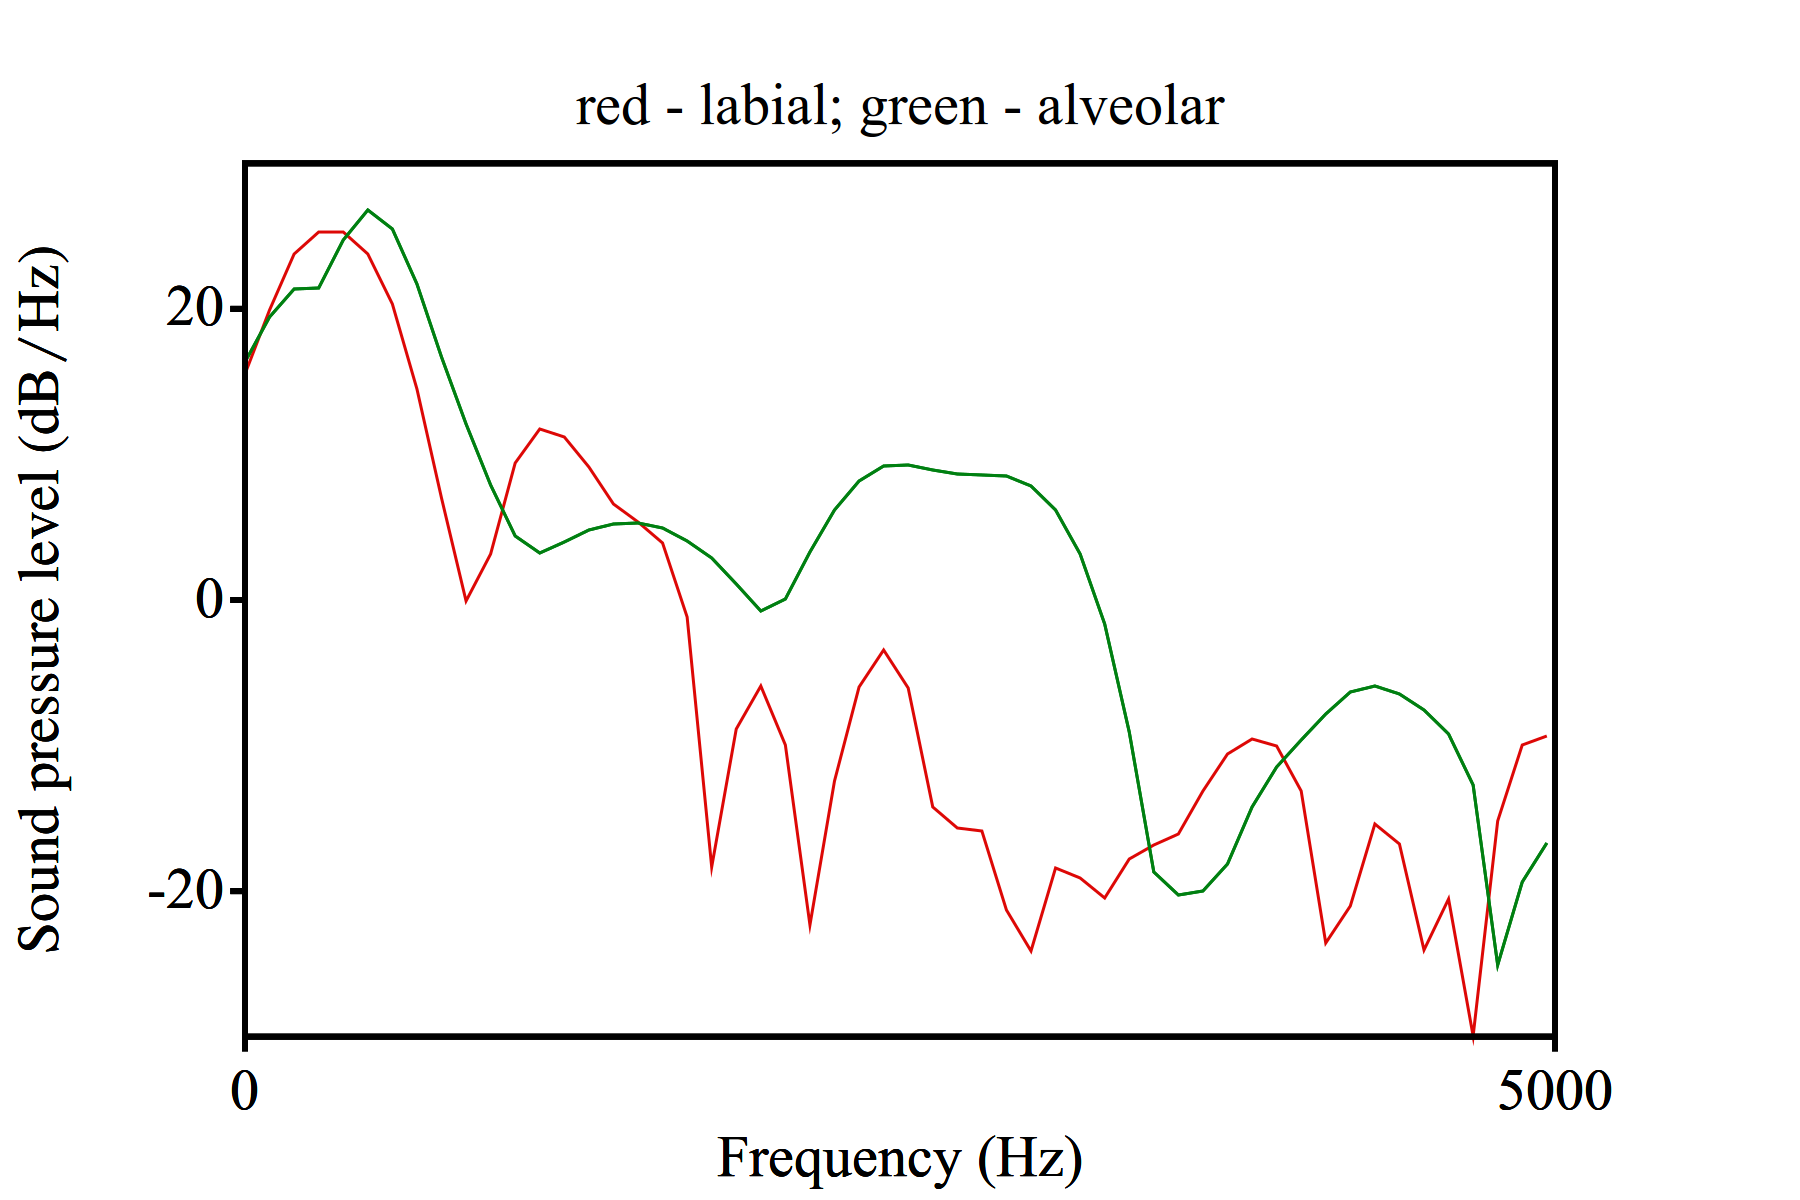
\includegraphics[width=\linewidth]{01-Spectral-Slice.png}
\end{frame}

\begin{frame}{Nasal Stops Acoustics: Spectral Slices}
\begin{itemize}
\item Praat Objects > Open Sound
\item View \& Edit
\item Find the middle of nasals or \textbf{one cycle}
\item Spectrum > View Spectrum slice \hfill \textbf{Ctrl+L}
\item Select Spectrum Slice object in Praat Object window
\item Praat Objects > Draw...\\
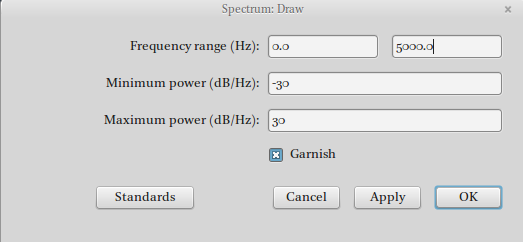
\includegraphics[width=0.8\linewidth]{02-params.png}
\item Spectrum > View Spectrum slice > Draw...
\end{itemize}
\end{frame}

\section{}
\begin{frame}
{\huge Thank you!\bigskip\\
\normalsize Please, don't hesitate to write me\\
agricolamz@gmail.com
\vspace{-130pt}}
\end{frame}
\end{document}
